\chapter{Sustancias puras y mezclas}\label{ch:g6:pure-substances-and-mixtures}

La etiqueta de una botella de agua mineral enumera una docena de
sustancias disueltas, con sus cantidades en miligramos por litro. El
agua que sale del purificador de un laboratorio no enumera ninguna. Las
dos son transparentes e incoloras, las dos quitan la sed y, sin embargo,
solo una de ellas es lo que un químico llama pura. Este capítulo da a la
palabra ``pura'' su sentido exacto y enseña a distinguir una \omterm{def:g6:pure-substances-and-mixtures:pure-substance}{sustancia
pura} de una \omterm{def:g6:pure-substances-and-mixtures:mixture}{mezcla} sin probar nada.

\begin{recall}
\omterm{def:g2:mixing-and-dissolving:mix}{Mezclar} es juntar cosas distintas; un sólido que se \omterm{def:g2:mixing-and-dissolving:dissolve}{disuelve} en agua
deja el líquido transparente, y ese líquido transparente es una
disolución (\cref{ch:g2:mixing-and-dissolving}). Las \omterm{def:g6:pure-substances-and-mixtures:mixture}{mezclas} se pueden
separar por \omterm{def:g3:separating-mixtures:sieve}{tamizado}, \omterm{def:g3:separating-mixtures:decant}{decantación}, \omterm{def:g3:separating-mixtures:filter}{filtración} y \omterm{def:g3:separating-mixtures:evaporate}{evaporación}
(\cref{ch:g3:separating-mixtures}). Todo material tiene propiedades que
se pueden poner a prueba: duro o blando, transparente o no, flota o se
hunde
(\cref{ch:g1:materials-around-us}).
\end{recall}

\section{Especies químicas y sustancias puras}

\begin{definition}[Especie química]\label{def:g6:pure-substances-and-mixtures:species}
Una \emph{especie química}\index{especie quimica@especie química} es una clase
concreta de sustancia, con su propio nombre y sus propias propiedades:
el agua, el azúcar, la sal, el oxígeno, el etanol (el alcohol del vino),
el hierro.
\end{definition}

\begin{definition}[Sustancia pura]\label{def:g6:pure-substances-and-mixtures:pure-substance}
Una \emph{sustancia pura}\index{sustancia pura} está formada por una
sola \omterm{def:g6:pure-substances-and-mixtures:species}{especie química} y nada más: el agua destilada, un cristal de
azúcar, un anillo de oro puro.
\end{definition}

\begin{definition}[Mezcla]\label{def:g6:pure-substances-and-mixtures:mixture}
Una \emph{mezcla}\index{mezcla} contiene varias \omterm{def:g6:pure-substances-and-mixtures:species}{especies químicas}. El
\omterm{def:g4:air-a-mixture-of-gases:air}{aire}, el agua del mar, el agua mineral, la leche, el granito y el zumo
de naranja son mezclas.
\end{definition}

\begin{remark}[Puro en el lenguaje de todos los días]\label{rem:g6:pure-substances-and-mixtures:everyday}
Un brik de ``zumo de naranja puro'' quiere decir que no se ha añadido
nada al zumo. Para un químico, el zumo sigue siendo una \omterm{def:g6:pure-substances-and-mixtures:mixture}{mezcla}: agua,
azúcares, ácidos, vitaminas, colorantes y aromas, muchas \omterm{def:g6:pure-substances-and-mixtures:species}{especies
químicas}. El ``agua pura de manantial'' también es una \omterm{def:g6:pure-substances-and-mixtures:mixture}{mezcla}: agua con
sales disueltas.
\end{remark}

\begin{omfigure}
\begin{tikzpicture}[font=\small, level distance=1.55cm,
    box/.style={draw=omDef, fill=omDef!6, rounded corners=2pt, align=center,
      inner sep=4pt},
    level 1/.style={sibling distance=7.2cm},
    level 2/.style={sibling distance=3.6cm},
    edge from parent/.style={draw, thick, omDef, ->}]
  \node[box] {materia}
    child {node[box] {sustancia pura\\ \footnotesize una especie química}
      child {node[box, draw=black!40, fill=white] {agua destilada,\\ sal, hierro}}}
    child {node[box] {mezcla\\ \footnotesize varias especies químicas}
      child {node[box] {homogénea\\ \footnotesize mismo aspecto en todas partes}
        child {node[box, draw=black!40, fill=white] {agua salada,\\ aire}}}
      child {node[box] {heterogénea\\ \footnotesize se ven sus partes}
        child {node[box, draw=black!40, fill=white] {agua turbia,\\ granito}}}};
\end{tikzpicture}

{\small Clasificación de la materia. Las cajas de abajo dan ejemplos de
cada clase.}
\end{omfigure}

\section{Mezclas homogéneas y heterogéneas}

\begin{definition}[Mezclas homogéneas y heterogéneas]\label{def:g6:pure-substances-and-mixtures:homogeneous}
Una \omterm{def:g6:pure-substances-and-mixtures:mixture}{mezcla} es una \emph{mezcla homogénea}\index{mezcla homogenea@mezcla homogénea}
cuando sus distintas partes no se pueden distinguir a simple vista, ni
siquiera con una lupa: tiene el mismo aspecto en todas partes. Es una
\emph{mezcla heterogénea}\index{mezcla heterogenea@mezcla heterogénea} cuando se ven al
menos dos partes distintas.
\end{definition}

\begin{example}[Cuatro mezclas]\label{ex:g6:pure-substances-and-mixtures:four}
El agua salada y el \omterm{def:g4:air-a-mixture-of-gases:air}{aire} son homogéneos: sus partes no se ven. El aceite
sobre el agua es heterogéneo: dos capas. El agua turbia es heterogénea:
en ella flotan granos que acaban depositándose. El zumo de naranja con
pulpa es heterogéneo: se ven los trocitos de pulpa.
\end{example}

\begin{omfigure}
\begin{tikzpicture}[font=\small, scale=1.15]
  \pic[transform shape] at (0,0) {beaker={0.7}{omWater!80}};
  \node[anchor=north, align=center] at (0,-0.15) {agua salada:\\ homogénea};
  \pic[transform shape] at (2.6,0) {beaker={0.7}{omWater!80}};
  \fill[yellow!55!orange!60] (1.8,1.05) rectangle (3.4,1.4);
  \draw[omGlass, line width=0.7pt] (1.8,1.05) -- (1.8,1.4) (3.4,1.05) -- (3.4,1.4);
  \node[anchor=north, align=center] at (2.6,-0.15) {aceite sobre agua:\\ heterogénea};
  \pic[transform shape] at (5.2,0) {beaker={0.7}{brown!25}};
  \foreach \x/\y in {4.6/0.3,4.9/0.7,5.3/0.5,5.6/1.0,5.0/1.1,5.4/0.2,5.8/0.6}
    \fill[brown!65] (\x,\y) circle (0.04);
  \fill[brown!60] (4.4,0) rectangle (6.0,0.12);
  \node[anchor=north, align=center] at (5.2,-0.15) {agua turbia:\\ heterogénea};
  \pic[transform shape] at (7.8,0) {beaker={0.7}{orange!45}};
  \foreach \x/\y in {7.3/0.35,7.6/0.8,8.0/0.5,8.3/1.0,7.7/1.15,8.2/0.25,7.45/0.65}
    \fill[orange!80!brown] (\x,\y) ellipse (0.08 and 0.03);
  \node[anchor=north, align=center] at (7.8,-0.15) {zumo con pulpa:\\ heterogénea};
\end{tikzpicture}

{\small Una \omterm{def:g6:pure-substances-and-mixtures:homogeneous}{mezcla homogénea} y tres \omterm{def:g6:pure-substances-and-mixtures:homogeneous}{mezclas heterogéneas}.}
\end{omfigure}

\begin{omfigure}
\begin{minipage}[b]{0.48\linewidth}\centering
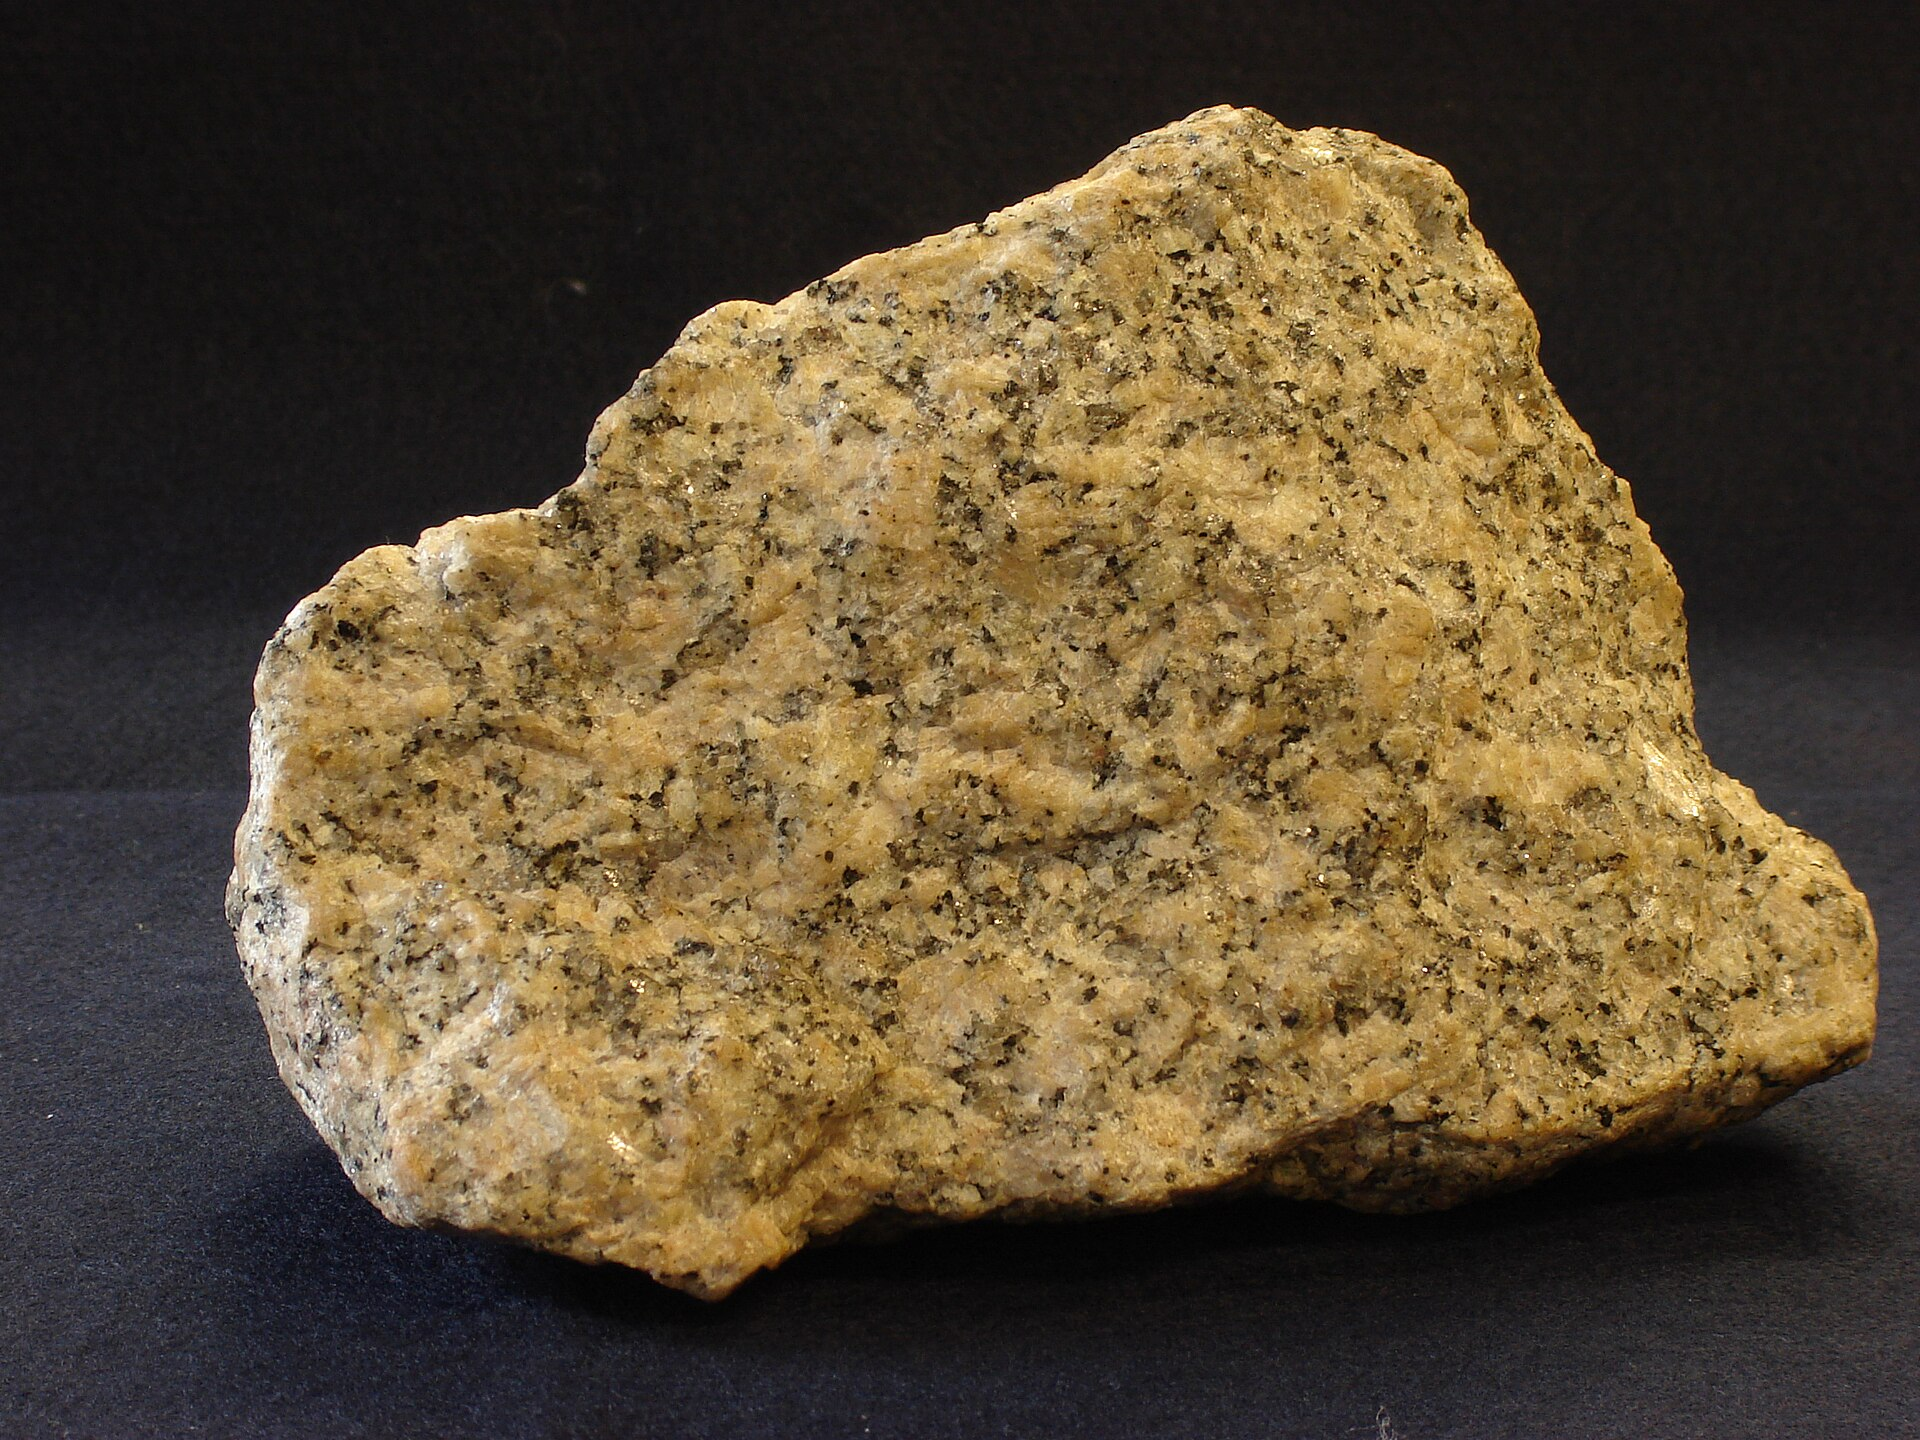
\includegraphics[width=\linewidth,height=4.6cm,keepaspectratio]{images/book1/granite.jpg}

{\small Granito: se ven granos de tres o cuatro minerales distintos. Un
sólido heterogéneo. Foto: Eurico Zimbres, CC BY-SA 2.0 br.}
\end{minipage}\hfill
\begin{minipage}[b]{0.48\linewidth}\centering
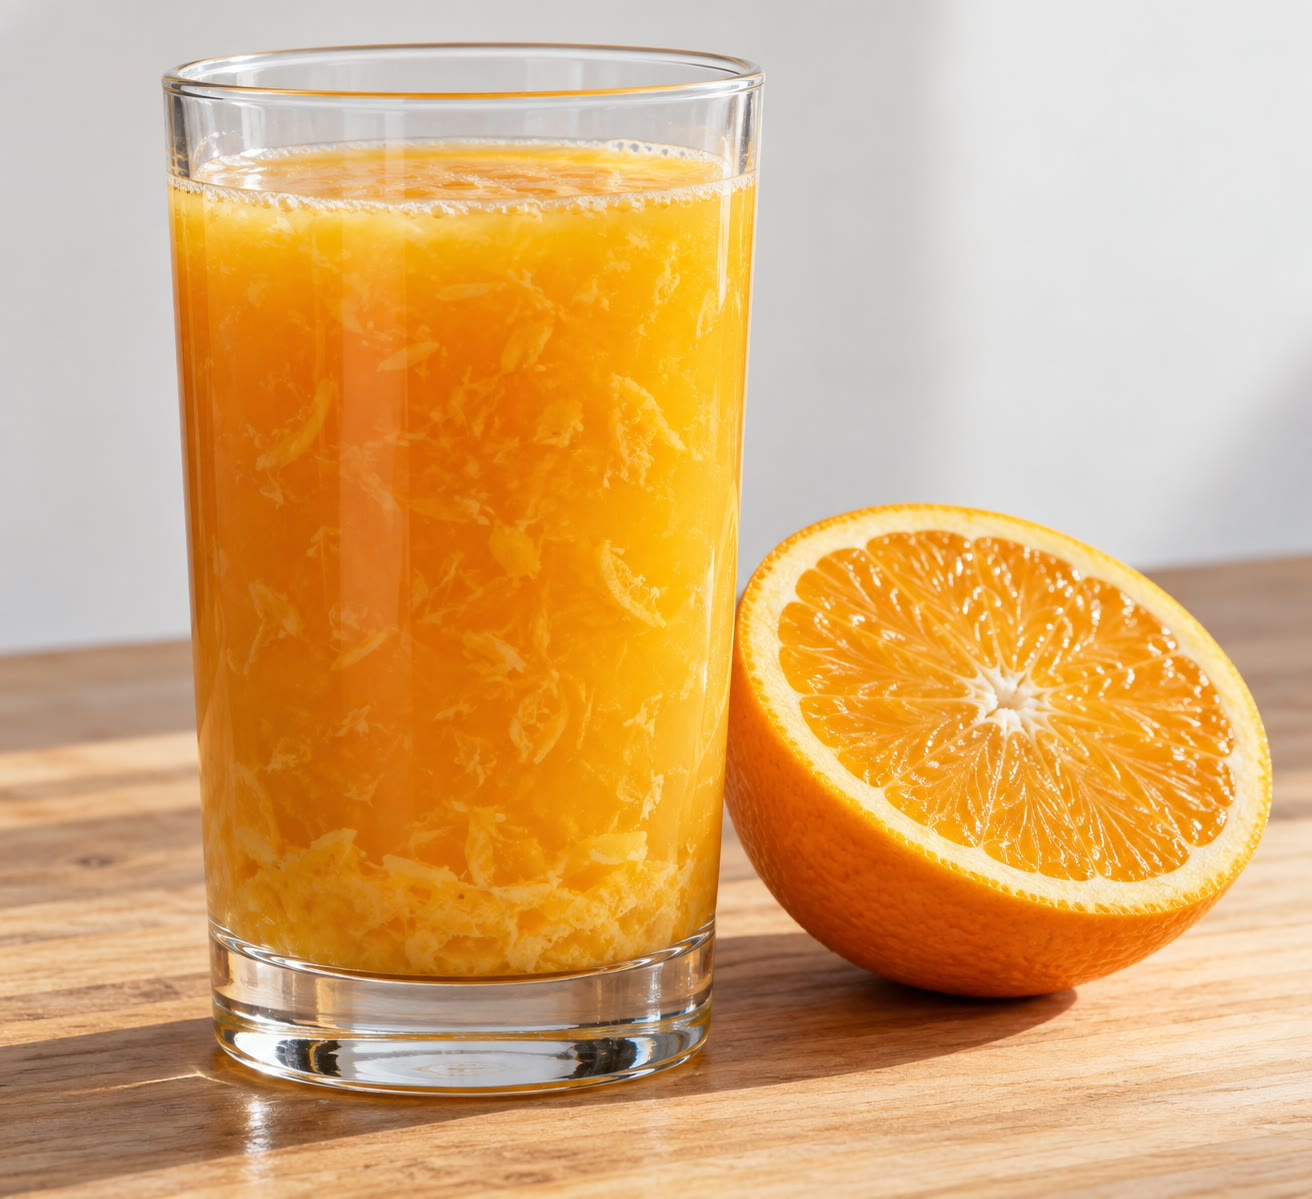
\includegraphics[width=\linewidth,height=4.6cm,keepaspectratio]{images/book1/ai/g6-orange-juice.jpg}

{\small Zumo de naranja con pulpa: una \omterm{def:g6:pure-substances-and-mixtures:homogeneous}{mezcla heterogénea}.}
\end{minipage}
\end{omfigure}

\begin{remark}[Homogénea no quiere decir pura]\label{rem:g6:pure-substances-and-mixtures:not-pure}
El agua salada se parece exactamente al agua pura. Mirar no basta para
distinguir una \omterm{def:g6:pure-substances-and-mixtures:pure-substance}{sustancia pura} de una \omterm{def:g6:pure-substances-and-mixtures:homogeneous}{mezcla homogénea}: hay que medir
algo.
\end{remark}

\section{Identificar una sustancia pura por sus constantes}

\begin{proposition}[Una sustancia pura tiene sus propias constantes]\label{prop:g6:pure-substances-and-mixtures:constants}
% ledger: mp:water, bp:water, bp:ethanol, mp:ethanol, rho:water, rho:ethanol, mp:NaCl, mp:Fe, rho:Fe
Cada \omterm{def:g6:pure-substances-and-mixtures:pure-substance}{sustancia pura} funde a una temperatura fija que le es propia,
hierve a una temperatura fija que le es propia (a presión normal) y
tiene su propia masa para un volumen dado, su densidad. Estos números
son sus constantes; el libro de física explica qué miden. Para algunas
\omterm{def:g6:pure-substances-and-mixtures:pure-substance}{sustancias puras}:
\begin{center}
\small
\begin{tabular}{lccc}
\hline
\omterm{def:g6:pure-substances-and-mixtures:pure-substance}{sustancia pura} & funde a & hierve a & masa de \qty{1}{cm^3} \\
\hline
agua & \qty{0}{\celsius} & \qty{100}{\celsius} & unos \qty{1.0}{g} \\
etanol & \qty{-114}{\celsius} & \qty{78}{\celsius} & \qty{0.79}{g} \\
propanona (acetona) & --- & \qty{56}{\celsius} & \qty{0.78}{g} \\
sal (cloruro de sodio) & \qty{801}{\celsius} & --- & \qty{2.17}{g} \\
hierro & \qty{1538}{\celsius} & --- & \qty{7.87}{g} \\
\hline
\end{tabular}
\end{center}
% ledger: bp:acetone, rho:acetone, rho:NaCl
\end{proposition}

\begin{proposition}[Una mezcla no tiene una temperatura de ebullición fija]\label{prop:g6:pure-substances-and-mixtures:mixture-boils}
Una \omterm{def:g6:pure-substances-and-mixtures:mixture}{mezcla} no hierve a una temperatura fija: el agua salada empieza a
hervir un poco por encima de \qty{100}{\celsius}, y su temperatura
sigue subiendo mientras hierve, porque el agua se va y la sal que queda
se concentra cada vez más.
\end{proposition}

\begin{method}[¿Es puro este líquido? ¿Cuál es?]\label{met:g6:pure-substances-and-mixtures:identify}
\begin{enumerate}
  \item Calentarlo, en el laboratorio, y leer su temperatura mientras
        hierve.
  \item Si la temperatura se mantiene fija, el líquido es probablemente
        una \omterm{def:g6:pure-substances-and-mixtures:pure-substance}{sustancia pura}: comparar esa temperatura con una tabla de
        constantes.
  \item Si la temperatura sigue subiendo, es una \omterm{def:g6:pure-substances-and-mixtures:mixture}{mezcla}.
  \item Confirmar con una segunda constante, por ejemplo la masa de un
        volumen conocido.
\end{enumerate}
\end{method}

\begin{inthelab}[Hervir agua salada]
El profesor calienta agua pura y agua salada una al lado de la otra,
cada una con un termómetro dentro. El agua pura hierve a
\qty{100}{\celsius} y se mantiene ahí mientras hierve. El agua salada
empieza a hervir un poco por encima de \qty{100}{\celsius}, y el
termómetro va subiendo poco a poco, minuto tras minuto.
\end{inthelab}

\section{El agua, pura y no tan pura}

\begin{example}[Cuatro aguas]\label{ex:g6:pure-substances-and-mixtures:waters}
% ledger: sea:salinity
\begin{itemize}
  \item El \textbf{agua destilada}, que se fabrica en un laboratorio, es
        casi una \omterm{def:g6:pure-substances-and-mixtures:pure-substance}{sustancia pura}: agua y nada más.
  \item El \textbf{agua del grifo} es una \omterm{def:g6:pure-substances-and-mixtures:homogeneous}{mezcla homogénea}: agua con
        pequeñas cantidades de sustancias disueltas (una gota secada
        sobre un plato oscuro deja un cerco blanco).
  \item El \textbf{agua mineral} es una \omterm{def:g6:pure-substances-and-mixtures:homogeneous}{mezcla homogénea} cuya etiqueta
        indica las sustancias disueltas, en miligramos por litro.
  \item El \textbf{agua del mar} es una \omterm{def:g6:pure-substances-and-mixtures:homogeneous}{mezcla homogénea} que contiene
        unos \qty{35}{g} de sales en cada kilogramo.
\end{itemize}
\end{example}

\begin{omfigure}
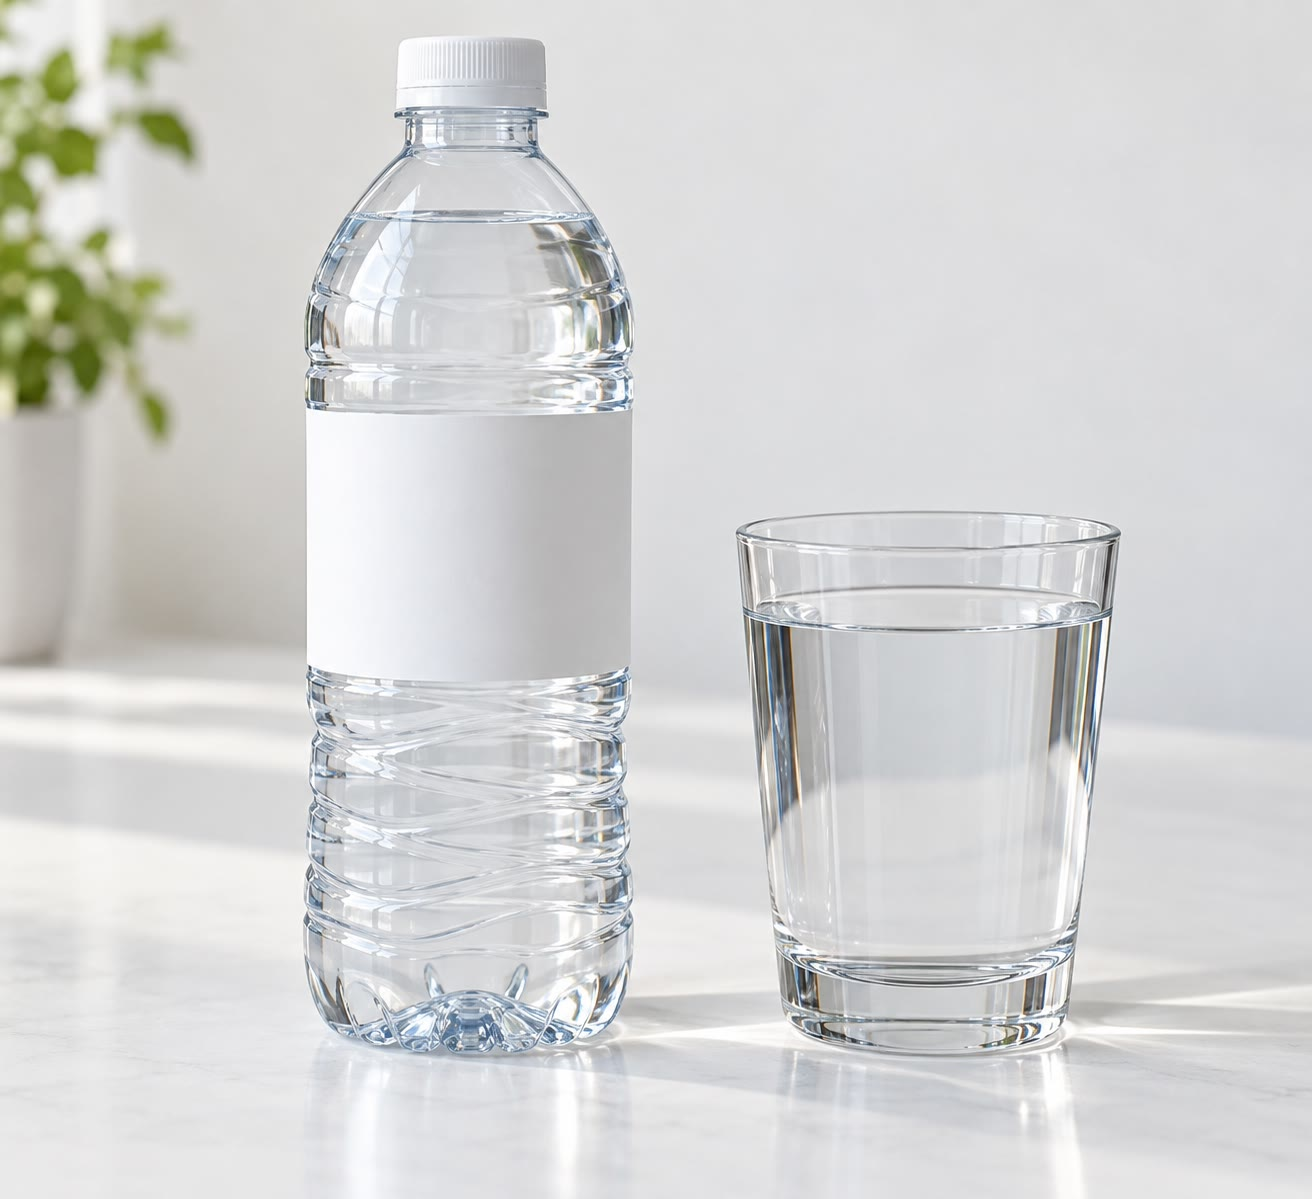
\includegraphics[width=0.5\linewidth]{images/book1/ai/g6-mineral-water.jpg}

{\small Una botella de agua mineral: transparente e incolora y, aun así,
una \omterm{def:g6:pure-substances-and-mixtures:mixture}{mezcla}.}
\end{omfigure}

\begin{example}[Leer la etiqueta de un agua mineral]\label{ex:g6:pure-substances-and-mixtures:label}
Una etiqueta indica: calcio \qty{78}{mg/L}, magnesio \qty{24}{mg/L},
sodio \qty{5}{mg/L}, hidrogenocarbonato \qty{357}{mg/L}, sulfato
\qty{10}{mg/L}, cloruro \qty{4}{mg/L}. (Estas cifras son un ejemplo.)
En un litro hay $78 + 24 + 5 + 357 + 10 + 4 = 478$\,mg de sustancias
disueltas, alrededor de medio gramo: muy poco al lado de los
\qty{1000}{g} de agua, pero suficiente para que sea una \omterm{def:g6:pure-substances-and-mixtures:mixture}{mezcla}.
\end{example}

\section{Ejercicios}

\begin{exercise}[$\star$]\label{exo:g6:pure-substances-and-mixtures:1}
¿\omterm{def:g6:pure-substances-and-mixtures:pure-substance}{Sustancia pura} o \omterm{def:g6:pure-substances-and-mixtures:mixture}{mezcla}? Agua destilada, \omterm{def:g4:air-a-mixture-of-gases:air}{aire}, agua del mar, un bloque
de hierro puro, leche, un cristal de azúcar.
\end{exercise}

\begin{exercise}[$\star$]\label{exo:g6:pure-substances-and-mixtures:2}
¿Homogénea o heterogénea? Agua salada, granito, aceite sobre agua, agua
del grifo, muesli.
\end{exercise}

\begin{exercise}[$\star$]\label{exo:g6:pure-substances-and-mixtures:3}
¿Qué es una \omterm{def:g6:pure-substances-and-mixtures:species}{especie química}? Da tres ejemplos.
\end{exercise}

\begin{exercise}[$\star$]\label{exo:g6:pure-substances-and-mixtures:4}
Un líquido hierve a \qty{78}{\celsius}, y su temperatura se mantiene
en \qty{78}{\celsius} mientras hierve. Usa la tabla de constantes para
proponer de qué líquido se trata.
\end{exercise}

\begin{exercise}[$\star$]\label{exo:g6:pure-substances-and-mixtures:5}
¿Por qué el ``zumo de naranja puro'' no es una \omterm{def:g6:pure-substances-and-mixtures:pure-substance}{sustancia pura} para un
químico?
\end{exercise}

\begin{exercise}[$\star\star$]\label{exo:g6:pure-substances-and-mixtures:6}
Un líquido empieza a hervir a \qty{100.5}{\celsius} y su temperatura
sube mientras hierve. ¿Es una \omterm{def:g6:pure-substances-and-mixtures:pure-substance}{sustancia pura}? ¿Qué podría ser?
\end{exercise}

\begin{exercise}[$\star\star$]\label{exo:g6:pure-substances-and-mixtures:7}
Mira la figura de los cuatro vasos de precipitados. ¿En qué vaso podría
un filtro separar las partes de la \omterm{def:g6:pure-substances-and-mixtures:mixture}{mezcla}? ¿En qué vaso no podría?
\end{exercise}

\begin{exercise}[$\star\star$]\label{exo:g6:pure-substances-and-mixtures:8}
Un cubo de metal de volumen \qty{10}{cm^3} tiene una masa de
\qty{78.7}{g}. ¿Cuál es la masa de \qty{1}{cm^3}? ¿Qué metal de la
tabla podría ser?
\end{exercise}

\begin{exercise}[$\star\star$]\label{exo:g6:pure-substances-and-mixtures:9}
Con la etiqueta de agua mineral del ejemplo, ¿qué porcentaje de la masa
disuelta es hidrogenocarbonato? Redondea al número entero más próximo.
\end{exercise}

\begin{exercise}[$\star\star$]\label{exo:g6:pure-substances-and-mixtures:10}
El agua del mar contiene unos \qty{35}{g} de sales por kilogramo. ¿Qué
masa de sales hay en un cubo de \qty{2}{kg} de agua del mar? ¿Qué
porcentaje de la masa del agua del mar es sal?
\end{exercise}

\begin{exercise}[$\star\star\star$]\label{exo:g6:pure-substances-and-mixtures:11}
Dos líquidos transparentes e incoloros parecen idénticos. Describe dos
medidas, hechas en un laboratorio, que mostrarían si son la misma
\omterm{def:g6:pure-substances-and-mixtures:pure-substance}{sustancia pura}.
\end{exercise}

\begin{exercise}[$\star\star\star$]\label{exo:g6:pure-substances-and-mixtures:12}
Una \omterm{def:g6:pure-substances-and-mixtures:mixture}{mezcla} está formada por \qty{90}{g} de agua y \qty{10}{g} de
etanol. ¿Qué porcentaje de su masa es etanol? ¿Se puede identificar con
la tabla de constantes? Explícalo.
\end{exercise}

\section{Problema: Tres líquidos incoloros}

\begin{problem}[{Problema de fin de semana --- tres matraces sin
etiqueta con un líquido transparente e incoloro, y las medidas que los
distinguen}]
\label{pb:g6:pure-substances-and-mixtures:1}
% ledger: bp:water, bp:ethanol, rho:water, rho:ethanol, rho:seawater, sea:salinity
Un auxiliar de laboratorio encuentra tres matraces, A, B y C, a los que
se les han caído las etiquetas. Los tres contienen un líquido
transparente e incoloro. El laboratorio solo usa tres líquidos así:
agua destilada, etanol y agua del mar traída de una salida de campo. El
auxiliar hace tres tipos de medidas, en el laboratorio.

\medskip
\noindent\textbf{Parte I --- Mirar.}
\begin{enumerate}
  \item Los tres líquidos parecen exactamente iguales. ¿Puede el
        auxiliar saber, mirándolos, cuáles son \omterm{def:g6:pure-substances-and-mixtures:pure-substance}{sustancias puras}?
        Explícalo.
  \item Si uno de ellos es una \omterm{def:g6:pure-substances-and-mixtures:mixture}{mezcla}, ¿es homogénea o heterogénea?
  \item ¿Qué tipo de medida puede mostrar que un líquido es una
        \omterm{def:g6:pure-substances-and-mixtures:pure-substance}{sustancia pura}?
\end{enumerate}

\medskip
\noindent\textbf{Parte II --- Medir.}
Se calienta cada líquido hasta que hierve. El líquido A hierve a
\qty{100}{\celsius} y su temperatura se mantiene ahí. El líquido B
hierve a \qty{78}{\celsius} y se mantiene ahí. El líquido C empieza a
hervir a \qty{100.6}{\celsius}, y su temperatura sigue subiendo
despacio. Después se pesan \qty{50.0}{mL} de cada líquido: A
\qty{49.8}{g}, B
\qty{39.5}{g}, C \qty{51.2}{g}.
\begin{enumerate}[resume]
  \item ¿Qué líquidos son \omterm{def:g6:pure-substances-and-mixtures:pure-substance}{sustancias puras}? ¿Cuál es una \omterm{def:g6:pure-substances-and-mixtures:mixture}{mezcla}?
  \item Con la tabla de constantes de este capítulo, nombra los
        líquidos A y B.
  \item Calcula la masa de \qty{1}{mL} (es decir, \qty{1}{cm^3}) de
        cada líquido.
  \item ¿Concuerdan estas masas con tu respuesta a la pregunta 5?
  \item ¿Por qué la temperatura del líquido C sigue subiendo mientras
        hierve?
\end{enumerate}

\medskip
\noindent\textbf{Parte III --- ¿Qué hay en el líquido C?}
Se dejan secar en un recipiente \qty{100}{mL} del líquido C. Cuando
toda el agua se ha ido, quedan \qty{3.5}{g} de cristales blancos.
\begin{enumerate}[resume]
  \item ¿Qué muestra este residuo sobre el líquido C?
  \item Con la masa de \qty{1}{mL} de C hallada en la pregunta 6,
        calcula la masa de \qty{100}{mL} de C y, después, el porcentaje
        de su masa que es sal (con un decimal).
  \item El agua del mar contiene unos \qty{35}{g} de sales en cada
        kilogramo. ¿Qué porcentaje es eso? Compáralo con la pregunta 10.
  \item Concluye: ¿cuántos gramos de sal contiene cada litro del
        líquido C, y es el líquido C el agua del mar?
\end{enumerate}
\end{problem}
